\documentclass{warpdoc}
\newlength\lengthfigure                  % declare a figure width unit
\setlength\lengthfigure{0.158\textwidth} % make the figure width unit scale with the textwidth
\usepackage{psfrag}         % use it to substitute a string in a eps figure
\usepackage{subfigure}
\usepackage{rotating}
\usepackage{pstricks}
\usepackage[innercaption]{sidecap} % the cute space-saving side captions
\usepackage{scalefnt}
\usepackage{bm}

%%%%%%%%%%%%%=--NEW COMMANDS BEGINS--=%%%%%%%%%%%%%%%%%%%%%%%%%%%%%%%%%%
\newcommand{\mfa}{\scriptscriptstyle}
\newcommand{\mfb}{\scriptstyle}
\newcommand{\mfc}{\textstyle}
\newcommand{\mfd}{\displaystyle}
\newcommand{\Cp}{{c_{p}}}
\newcommand{\Cphi}{{C_{\phi}}}
\newcommand{\nd}{d}
\newcommand{\CFL}{{\rm CFL}}
\newcommand{\xiverge}{{\xi_{\rm verge}}}
\newcommand{\kdiv}{{k_{\rm div}}}
\newcommand{\varphiverge}{{\varphi_{\rm verge}}}
\newcommand{\ximax}{{\xi_{\rm max}}}
\newcommand{\turb}{_{\rm t}}
\newcommand{\mut}{\mu\turb}
\newcommand{\Mt} {{\rm M}\turb}
\newcommand{\Prt}{{\rm Pr}\turb}
\newcommand{\krodel}{\delta^{\rm K}}
\newcommand{\mc}{\multicolumn}
\newcommand{\cc}{\multicolumn{1}{c}}
\newcommand{\ie}{{\it i.e.}}
\newcommand{\etal}{{\it et al.}}
\newcommand{\etc}{{\it etc.}}
\newcommand{\apriori}{{\it a priori}}
\newcommand{\pseudot}{\tau}
\newcommand{\Cv}{{C_{\rm v}}}
\newcommand{\MC}{{\rm M}_{\rm c}}
\newcommand{\Cf}{C_{\rm f}}
\newcommand{\Sct}{{{\rm Sc}_{\rm t}}}
\newcommand{\ns}{{{n}_{\rm s}}}
\newcommand{\dd}{\; {\rm d}}
\newcommand\frameeqn[1]{\fbox{$\displaystyle #1$}}
\newcommand{\ordi}{\; {\rm d}}
\newcommand{\mdot}{\dot{m}}
\newcommand{\mdotengine}{\dot{m}_{\rm engine}}
\newcommand{\mdotairengine}{\dot{m}_{\rm air,~engine}}
\newcommand{\thetac}{\theta_{\rm c}}
\newcommand{\thetae}{\theta_{\rm e}}
\newcommand{\Lf}{L_{\rm f}}
\newcommand{\etam}{\eta_{\rm m}}
\newcommand{\yplus}{y^{+}}
\newcommand{\alb}{\vspace{0.1cm}\\} % array line break
\newcommand{\Sda}{S_{{\rm d}A}}
\newcommand{\Schem}{S_{\rm chem}}
\newcommand{\Smhd}{S_{\rm MHD}}
\newcommand{\Sturb}{S_{\rm turb}}
\newcommand{\betae}{\beta_{\rm e}}
\newcommand{\sigmatilde}{\widetilde{\sigma}}
\newcommand{\bigfrac}{\mfd\frac}
\newcommand{\etotal}{e_{\rm tot}}
\newcommand{\rhocharge}{\rho_{\rm c}}
\newcommand{\Bdipole}{B_{\rm d}}
\renewcommand{\fontsizetable}{\footnotesize\scalefont{1.0}}
\renewcommand{\fontsizefigure}{\footnotesize}
\renewcommand{\vec}[1]{\bm{#1}}
\setcounter{tocdepth}{3}
\let\citen\cite

%%%%%%%%%%%%%=--NEW COMMANDS BEGINS--=%%%%%%%%%%%%%%%%%%%%%%%%%%%%%%%%%%

\setcounter{tocdepth}{3}

%%%%%%%%%%%%%=--NEW COMMANDS ENDS--=%%%%%%%%%%%%%%%%%%%%%%%%%%%%%%%%%%%%



\author{
  Bernard Parent
}

\email{
  bparent@princeton.edu
}

\department{
  Dept. of Mechanical and Aerospace Engineering
}

\institution{
  Princeton University
}

\title{
  Magnetohydrodynamics (MHD) Effects on Quasi-1D Compressible Flow
}

\date{
  October 2002 -- February 2005
}

%\setlength\nomenclaturelabelwidth{0.13\hsize}  % optional, default is 0.03\hsize
%\setlength\nomenclaturecolumnsep{0.09\hsize}  % optional, default is 0.06\hsize

\nomenclature{
  \begin{nomenclaturelist}{Roman symbols}
   \item[$\vec{\bf A}$] origin of the magnet dipole moment
   \item[$A$]         cross-sectional area, $\rm m^2$
   \item[$\Bdipole$]  strength of the magnetic dipole, $\rm T$
   \item[$B_z$]         $z$-component of the magnetic field vector, $\rm N/A \, m$, $\rm T$
   \item[$\vec{\bf B}$] point along the dipole axis of symmetry, at a distance $r_{\rm ref}$
                        from point $\vec{\bf A}$
   \item[$\vec{B}$]         magnetic field vector, $\rm N/A \, m$, $\rm T$
   \item[$\overline{B}_i$]  ratio between the $i$th component of magnetic field vector and
                      the magnetic field magnitude
   \item[$|\vec{B}|$] magnitude of the magnetic field vector
   \item[$\vec{\bf C}$] point in the plane including the dipole axis of symmetry and point
                      $\vec{\bf P}$
   \item[$c_k$]       mass fraction of $k_{\rm th}$ species
   \item[$\Cp$]       specific heat at constant pressure, $\rm J/kg\, K$
   \item[$\Cphi$]     constant part of the fictitious unsteady term for $\phi$,
                      set to $1.0 \rm s^2 \, A^2 / N \, m^4$
   \item[$d$]         number of dimensions
   \item[$d_{\rm w}$] distance between the wall and the near-wall node
   \item[$e$]         internal energy of the gas, $\rm m^2/s^2$
   \item[$\etotal$]   total energy of the gas, $\rm m^2/s^2$
   \item[$E_y$]   $y$-component of the electric field vector, $\rm N/A \, s$, $\rm V/m$
   \item[$\vec{E}$]   electric field vector, $\rm N/A \, s$, $\rm V/m$
   \item[$F$]         convection flux vector
   \item[$G$]         diffusion variables vector
   \item[$h_k$]       partial enthalpy of $k_{\rm th}$ species
   \item[$i_r$]       unit vector of the applied magnetic field in the radial direction
   \item[$i_\theta$]       unit vector of the applied magnetic field in the $\theta$ direction
   \item[$J$]         metric Jacobian, $\rm 1/m$
   \item[$J_y$]         $y$ component of the current density vector, $\rm A/m^2$
   \item[$\vec{J}$]   current density vector, $\rm A/m^2$
   \item[$k$]         turbulence kinetic energy, TKE, $\rm m^2/s^2$
   \item[$K$]         diffusion matrix
   \item[$K$]         electric load factor, $E_y/qB_z$
   \item[$\Mt$]       turbulence Mach number, $\sqrt{2k}/a$
   \item[$\ns$]       number of species
   \item[$\vec{\bf P}$] point where the magnetic field vector is determined
   \item[$P$]         pressure, $\rm Pa$, $\rm N/m^2$
   \item[$P_k$]       production term of the TKE equation
   \item[$\Prt$]      turbulent Prandtl number
   \item[$Q$]         vector of conservative variables
   \item[$u$]         flow speed, $\rm m/s$
   \item[$R$]         residual vector
   \item[$R_k$]       gas constant of $k_{\rm th}$ species
   \item[$r$]         distance to the magnetic dipole center
   \item[$r_{\rm ref}$]         distance between the dipole center and an arbitrary point
                      on the dipole axis of symmetry where the magnitude of the magnetic field
		      is $\Bdipole$
   \item[$\Schem$]    source terms related to chemistry
   \item[$\Sct$]      turbulent Schmidt number
   \item[$\Sda$]      source terms related to the change in cross-sectional area
   \item[$\Smhd$]     source terms related to MHD
   \item[$\Sturb$]    source terms related to turbulence
   \item[$T$]         temperature, $\rm K$
   \item[$\vec{V}$]   velocity vector, $\rm m/s$
   \item[$W_k$]       chemical source term for $k_{\rm th}$ species
   \item[$X$]         non-dimensional computational coordinate
   \item[$X_{m,n}$]   $\partial X_m / \partial x_n$
   \item[$x,~y,~z$]   physical coordinates, $\rm m$
  \end{nomenclaturelist}


  \begin{nomenclaturelist}{Greek symbols}
   \item[$\alpha_{ij}$]  commonly used term in the diffusion matrix $K$
   \item[$\beta_{ij}^{mn}$]  commonly used term in the diffusion matrix $K$
   \item[$\betae$]    Hall parameter for the electrons
   \item[$\chi_{ij}$]  commonly used term in the diffusion matrix $K$
   \item[$\gamma$]  ratio of the specific heats
   \item[$\phi$]      electric field potential, V
   \item[$\epsilon$]      dissipation rate of the TKE
   \item[$\epsilon_0$]   permittivity of free space, $8.854 \times 10^{-12}~{\rm farad/m}$,
                         $0.079686~{\rm m/m}$
   \item[$\rho$]      density, $\rm kg/m^3$
   \item[$\rhocharge$]      charge density, $\rm coulomb/m^3$
   \item[$\krodel_{i,j}$]   Kronecker delta, equals 1 if $i=j$, 0 otherwise
   \item[$\sigma$]    electrical conductivity, $\rm 1/ohm \, m$, $\rm mho/m$, $\rm S/m$,
                      $\rm A^2 s/ N\, m^2$
   \item[$\sigmatilde$]   electrical conductivity tensor, $\rm 1/ohm \, m$, $\rm mho/m$, $\rm S/m$,
                      $\rm A^2 s/ N\, m^2$
   \item[$\mu$]       viscosity, $\rm kg/ms$
   \item[$\mu_k^\star$]       diffusion coefficient part of the TKE equation $\rm kg/ms$
   \item[$\mu_\omega^\star$]  diffusion coefficient part of the specific dissipation
                      rate equation $\rm kg/ms$
   \item[$\mu_0$]      permeability of free space, $4 \pi \times 10^{-7}~{\rm henry/m}$,
                       $1.398637 \times 10^{-16}~{\rm s^2/m^2}$
  \end{nomenclaturelist}

  \begin{nomenclaturelist}{Subscripts}
   \item[$t$]      turbulent
   \item[$w$]      wall
   \item[$x,y,z$]  the first, second, and third component of the vector
                   in Cartesian coordinates
  \end{nomenclaturelist}
}


\abstract{
The goal of this report is to present the magnetohydrodynamics equations for quasi-1D flow and to outline some derivations of interest.
}

\begin{document}
  \pagestyle{headings}
  \pagenumbering{arabic}
  \setcounter{page}{1}
%%  \maketitle
  \makewarpdoctitle
  \makeabstract
  \tableofcontents
%%  \makenomenclature
%%  \listoftables
%%  \listoffigures




























\section{Introduction and motivation}

There has been a substantial recent interest in how to
improve the performance of hypervelocity flight vehicles with MHD. One such application
is the bypass of the flow mechanical energy from the inlet to the nozzle (such as in
project AJAX \cite{aiaaconf:1996:gurijanov,aiaaconf:2001:kuranov} or
others \cite{aiaabook:2001:vatazhin,jpp:2001:litchford}).
By bypassing some of the flow mechanical energy around the combustor, it is hoped
that the flow velocity in the combustor can be reduced to subsonic speeds while
maintaining the maximum static temperature at the combustor entrance to a reasonable
value. However, to the author's knowledge, a numerical or experimental study of this MHD-ramjet
showing a benefit over the conventional ramjet (without energy bypass) has not yet
appeared in the open litterature. One of the goals of the present report is hence to
investigate on whether the flow can be slowed to subsonic speeds while maintaining
the temperature to below a certain limit through the use of MHD energy extraction.

Other
possible applications of MHD to hypersonic flight include the observed drag reduction
over blunt bodies when an external magnetic field is applied to a conducting incoming
flow (see Ref.\ \cite{aiaa:2002:shang} for instance), and the control of the shock positioning
in a scramjet inlet to achieve shock-on-lip condition over a relatively wide Mach number range
\cite{aiaaconf:2002:shneider} while keeping the geometry fixed.

There is also
a considerable interest in MHD as a means to generate electrical
power aboard a high-speed flight vehicle. The drastically high mechanical
energy of the flow at a high Mach number can be converted to electrical energy
through a MHD generator at the expense of a sudden reduction in flight speed.
Preliminary estimates show that a power
of hundreds of thousands of megawatts per cubic meter could be produced in such a way
\cite{aiaaconf:2002:thibodeaux}. The power
could then be used to feed a high-energy laser aimed at ground, air, or space targets. No
other known source of energy (except nuclear) could generate this type of power.

Yet other advantages of the presence of a weakly ionized flow in a hypersonic propulsion
device include the possible increase in mixing and ignition \cite{aiaaconf:2002:bocharov}
or the decrease in induction time of the burning
of a kerosene-air mixture \cite{aiaaconf:2002:klimov}. The latter is
particularly important to the possibility of using kerosene in small-size scramjets due
to the very high kerosene/air mixture induction time for burning as compared to a mixture
of hydrogen and air.



%%%%%%%%%%%%%%%%%%%%%%%%%%%%%%%%%%%%%%%%%%%%%%%%%%%%%%%%%%%%%%%%%%%%%%%%%%%%%%%%%%%%%%%%%%%%%%%%%%%%%%
%%%%%%%%%%%%%%%%%%%%%%%%%%%%%%%%%%%%%%%%%%%%%%%%%%%%%%%%%%%%%%%%%%%%%%%%%%%%%%%%%%%%%%%%%%%%%%%%%%%%%%
%%%%%%%%%%%%%%%%%%%%%%%%%%%%%%%%%%%%%%%%%%%%%%%%%%%%%%%%%%%%%%%%%%%%%%%%%%%%%%%%%%%%%%%%%%%%%%%%%%%%%%


\section{Quasi-one-dimensional perfect-gas flow}

This section is focused on studying the impact of the MHD source terms on the flow for the case
of quasi-one-dimensional formulation. This can be done numerically by trying out several
configurations, but this can also be done analytically, as is performed now.

\subsection{Governing equations}

%
Let's
first write down the steady-state quasi-one-dimensional MHD equations for a calorically and thermally
perfect gas, without any chemistry:
%
\begin{equation}
  \frac{\ordi}{\ordi x}
     \left[
      \begin{array}{@{}c@{}}
        A {\rho} u \alb
        A {\rho} u^2 +  A P\alb
        A {\rho} u \left(e+u^2/2\right)+ A u P \alb
      \end{array}
    \right]
  -\left[
      \begin{array}{@{}c@{}}
      0 \alb
      P \ordi A / \ordi x\alb
      0 \alb
      \end{array}
   \right]
  -\left[
      \begin{array}{@{}c@{}}
      0 \alb
      A (\vec{J} \times \vec{B})_x\alb
      A (\vec{J}\cdot \vec{J}/\sigma + \vec{V} \cdot (\vec{J}\times \vec{B}))\alb
      \end{array}
   \right]=0
\end{equation}
%
where the energy source term in the last term on the LHS comes from the substitution
of $\vec{E}$ in the generalized Ohm's law (\ie\ $\vec{E}=\vec{J}/\sigma + \vec{B} \times \vec{V}$)
to $\vec{E} \cdot \vec{J}$:
%
\begin{displaymath}
  \vec{E} \cdot \vec{J} = (\vec{J}/\sigma + \vec{B} \times \vec{V}) \cdot \vec{J}\alb
    =\vec{J} \cdot \vec{J} / \sigma + \vec{V} \cdot (\vec{J} \times \vec{B})~.
\end{displaymath}
%
\begin{figure}
   \fontsizefigure\center
   \psfrag{x}[lb][lb][1][0]{$x$}
   \psfrag{y}[rb][rb][1][0]{$y$}
   \psfrag{z}[rt][rt][1][0]{$z$}
   \psfrag{E}[l][l][1][0]{$E_y$}
   \psfrag{B}[rt][rt][1][0]{$B_z$}
   \psfrag{j}[rb][rb][1][0]{$J_y$}
   \psfrag{dx}[rb][rb][1][0]{d$x$}
   \psfrag{flow}[rb][rb][1][0]{flow}
   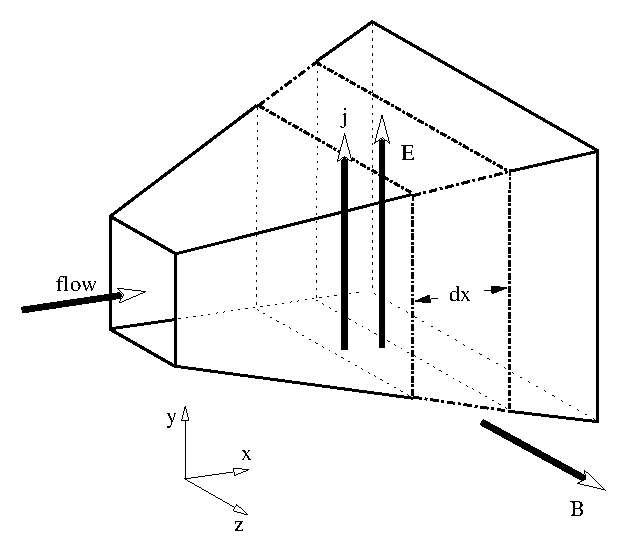
\includegraphics[width=4.0\lengthfigure]{setup.eps}
\caption{Problem setup, showing a typical flow section with the sidewalls
         insulated and the lower and upper walls having a potential difference in the direction of
	 the current flow.}
\label{fig:setup}
\end{figure}
For a current, electric field, and magnetic field positioned as in Figure
\ref{fig:setup} we can rewrite the governing equations as:
%
\begin{equation}
  \frac{\ordi}{\ordi x}
     \left[
      \begin{array}{@{}c@{}}
        A {\rho} u \alb
        A {\rho} u^2\alb
        A {\rho} u \left(h+u^2/2\right)\alb
      \end{array}
    \right]
  +\left[
      \begin{array}{@{}c@{}}
      0 \alb
      A \ordi P / \ordi x\alb
      0 \alb
      \end{array}
   \right]
  -\left[
      \begin{array}{@{}c@{}}
      0 \alb
      A J_y B_z\alb
      A (J_y^2/\sigma + u J_y B_z)\alb
      \end{array}
   \right]=0
\end{equation}
%
Substituting the continuity equation in the momentum and energy equations, the latter
becomes:
%
\begin{eqnarray}
\frac{\ordi}{\ordi x} A \rho u &=& 0 {\rm ~~~~(continuity)}\label{eqn:continuity}\alb
  \rho u \frac{\ordi u}{\ordi x} +  \frac{\ordi P}{\ordi x} -  J_y B_z &=&0 {\rm ~~~~(momentum)}\label{eqn:momentum}\alb
  \rho u \frac{\ordi}{\ordi x} \left( h+u^2/2 \right) - (J_y^2/\sigma + u J_y B_z)&=&0 {\rm ~~~~(energy)}\label{eqn:energy}
\end{eqnarray}
%



\subsection{Increase of pressure wrt temperature}

In this subsection, we seek a relationship to find the value of $\ordi T / \ordi P$
at a specific point in the duct. Let's isolate $\ordi u / \ordi x$ in the momentum
equation, Eq.\ (\ref{eqn:momentum}), and substitute it in the energy equation, Eq.\ (\ref{eqn:energy}):
%
\begin{equation}
\rho u \frac{\ordi h}{\ordi x}
- u \frac{\ordi P}{\ordi x} + u J_y B_z
- (J_y^2/\sigma + u J_y B_z)=0~,
\end{equation}
%
and, reformatting:
%
\begin{equation}
\rho u \Cp \frac{\ordi T}{\ordi x}
- u \frac{\ordi P}{\ordi x}
- J_y^2/\sigma=0~.
\end{equation}
%
Now, let's divide each term by $u \ordi P / \ordi x$:
%
\begin{equation}
\rho \Cp \frac{\ordi T}{\ordi P}
- 1
- \frac{\ordi x }{\ordi P} \frac{J_y^2}{u\sigma}=0~,
\end{equation}
%
or,
%
\begin{equation}
\rho \Cp \frac{\ordi T}{\ordi P}
= 1
+ \frac{\ordi x }{\ordi P} \frac{J_y^2}{u\sigma}~.
\end{equation}
%
Defining the electrical load factor $K$ such that $E_y=K u B_z$, then from the generalized Ohm's
law, we get an expression for the current corresponding to $J_y=(K-1)\sigma u B_z$. Substituting
this in the latter equation yields
%
\begin{equation}
\frameeqn{
\frac{\ordi T}{\ordi P}
= \frac{1}{\rho \Cp} \left[
1
+ \frac{(K-1)^2 \sigma u B_z^2}{\ordi P / \ordi x}
\right]}~.
\label{eqn:dTdP}
\end{equation}
%
Equation (\ref{eqn:dTdP}) shows that \emph{in a compression process (\ie\ for $\ordi P / \ordi x > 0$)
the rise in temperature accompanying a rise in pressure will always be greater when
a magnetic field is present than when it is not.} In other words, whether heat is extracted or
added to the flow, whether the flow is subsonic or supersonic, the presence of a magnetic field
will \emph{always} yield a higher final static temperature for the same pressure ratio through
the compression process. Another way to look at Eq.\ (\ref{eqn:dTdP}) is by integrating both
sides on the compression/expansion path:
%
\begin{equation}
\frac{\ordi T}{T}
= \frac{R}{\Cp} \frac{\ordi P}{P}
\left[ 1 + \frac{(K-1)^2 \sigma u B_z^2}{\ordi P / \ordi x}
\right]~,
\end{equation}
%
%
or,
%
\begin{equation}
\frac{\gamma}{\gamma-1}\frac{\ordi T}{T}
=  \frac{\ordi P}{P}
+ \frac{(K-1)^2 \sigma u B_z^2}{P} \ordi x~,
\end{equation}
%
Now, integrate both sides along the flow path, going from position 1 to position 2:
%
\begin{equation}
\int \frac{\gamma}{\gamma-1}\frac{\ordi T}{T}
= \int \frac{\ordi P}{P}
+ \int \frac{(K-1)^2 \sigma u B_z^2}{P} \ordi x~,
\end{equation}
%
or,
%
\begin{equation}
\frac{\gamma}{\gamma-1} \ln \left( \frac{T_2}{T_1} \right)
= \ln \left( \frac{P_2}{P_1} \right) + \int_{x_1}^{x_2} \frac{(K-1)^2 \sigma u B_z^2}{P} \ordi x
\end{equation}
%
or,
%
\begin{equation}
\ln \left( \frac{T_2}{T_1} \right)
=   \frac{\gamma-1}{\gamma} \ln \left( \frac{P_2}{P_1} \right)
  + \frac{\gamma-1}{\gamma}\int_{x_1}^{x_2} \frac{(K-1)^2 \sigma u B_z^2}{P} \ordi x
\end{equation}
%
%
\begin{equation}
\frac{T_2}{T_1}
= \exp \left[  \frac{\gamma-1}{\gamma} \ln \left( \frac{P_2}{P_1} \right)
  + \frac{\gamma-1}{\gamma}\int_{x_1}^{x_2} \frac{(K-1)^2 \sigma u B_z^2}{P} \ordi x \right]
\end{equation}
%
%
\begin{equation}
\frac{T_2}{T_1}
= \exp \left[  \frac{\gamma-1}{\gamma} \ln \left( \frac{P_2}{P_1} \right) \right]
  \exp \left[ \frac{\gamma-1}{\gamma}\int_{x_1}^{x_2} \frac{(K-1)^2 \sigma u B_z^2}{P} \ordi x \right]
\end{equation}
%
%
\begin{equation}
\frameeqn{
\frac{T_2}{T_1}
= \left( \frac{P_2}{P_1} \right)^\frac{\gamma-1}{\gamma}
  \exp \left[ \frac{\gamma-1}{\gamma}\int_{x_1}^{x_2} \frac{(K-1)^2 \sigma u B_z^2}{P} \ordi x \right]
}
\label{eqn:T2overT1}
\end{equation}
%
Again, it can be observed that \emph{along the flow path, for a specified pressure ratio $P_2/P_1$,
the temperature ratio $T_2/T_1$ will always be higher when a magnetic field
is present.} This is due to the integral part of the second term on the RHS of
Eq.\ (\ref{eqn:T2overT1}) always yielding a positive value since all the terms except for $u$
in the integral are always positive. When $u$ is positive, then $x_2$ is consequently greater
than $x_1$, and when $u$ is negative then $x_2$ is consequently smaller than $x_1$, which \emph{always}
yields a positive integral in the end. Since the integral part of the second term is always
positive, then the second term will always be greater or equal to 1, hence always yielding a
temperature ratio greater or equal to the one obtained without any magnetic field
interaction.




\subsection{Isothermal path}

For a constant temperature process, $\ordi h / \ordi x =0$. The momentum equation
[Eq.\ (\ref{eqn:momentum})] and the energy equation [Eq.\ (\ref{eqn:energy})] become,
%
\begin{equation}
     A\rho u^2 \frac{\ordi}{\ordi x}
     \left[
      \begin{array}{@{}c@{}}
         u\alb
         u\alb
      \end{array}
    \right]
  +\left[
      \begin{array}{@{}c@{}}
      A u \ordi P / \ordi x\alb
      0 \alb
      \end{array}
   \right]
  -\left[
      \begin{array}{@{}c@{}}
      A u J_y B_z\alb
      A (J_y^2/\sigma + u J_y B_z)\alb
      \end{array}
   \right]=0
\end{equation}
%
For the latter to hold true on a isothermal path, then:
%
\begin{equation}
A u \frac{\ordi P}{\ordi x} = -A J_y^2 / \sigma
\end{equation}
%
and, since $P=\rho R T$, we can write:
%
\begin{equation}
A u R T \frac{\ordi \rho}{\ordi x} = -A J_y^2 / \sigma
\end{equation}
%
but, from the continuity equation, $A u \ordi \rho / \ordi x=-\rho \ordi A u / \ordi x$:
%
\begin{equation}
P \frac{\ordi A u}{\ordi x} = A J_y^2 / \sigma
\end{equation}
%
%
\begin{figure}
   \fontsizefigure\center
   \psfrag{X}[t][t][1][0]{$K$}
   \psfrag{Y}[b][b][1][0]{$\mfd (K-1)^2 \left[ (\gamma M^2 -1) - \mfd\frac{1}{K-1} \right]$}
   \psfrag{A}[l][l][1][0]{$0.5$}
   \psfrag{B}[r][r][1][0]{$M=2$}
   \psfrag{C}[r][r][1][0]{$6$}
   \psfrag{D}[l][l][1][0]{$10$}
   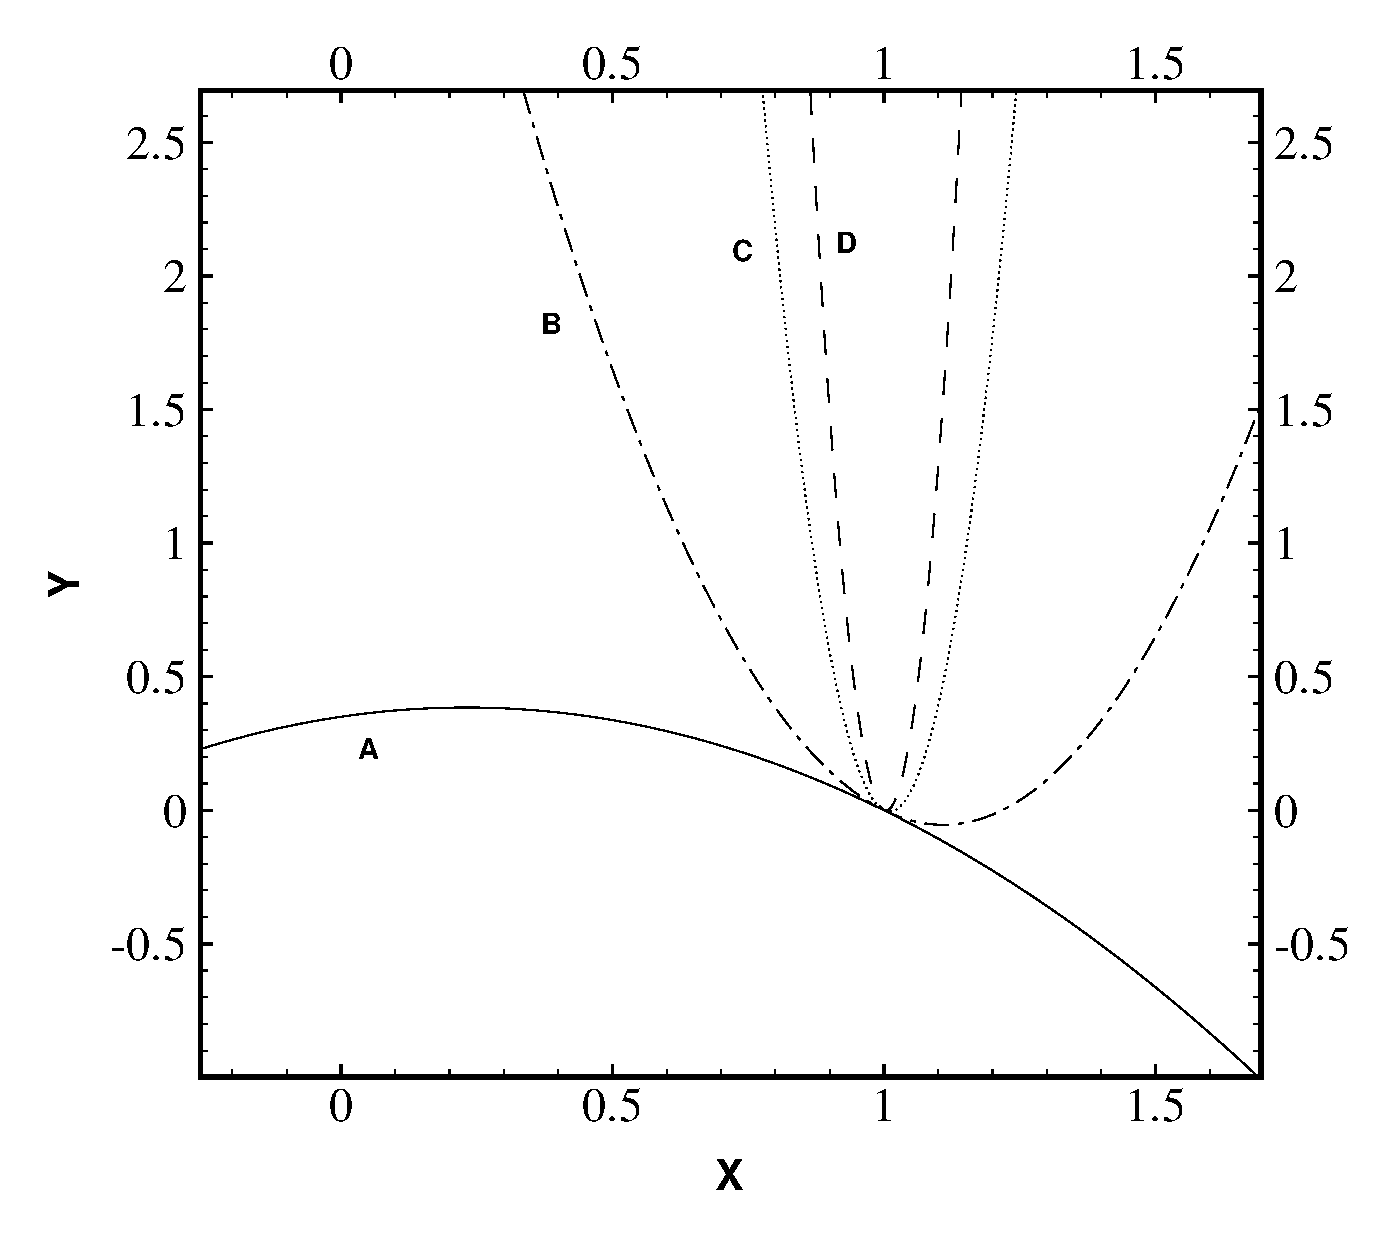
\includegraphics[width=4.36\lengthfigure]{dAdx.eps}
\caption{Change in cross-sectional area versus the electrical load factor $K$
         for different flow Mach numbers for the special case of isothermal compression/expansion
	 for $\gamma=1.4$.}
\label{fig:dAdx}
\end{figure}
%
%
\begin{equation}
P u \frac{\ordi A }{\ordi x}+P A \frac{\ordi u }{\ordi x} = A J_y^2 / \sigma
\end{equation}
%
but, from the conservation of energy on an isothermal path, $\ordi u / \ordi x = \frac{1}{\rho u ^2}(J_y^2/\sigma+u J_y B_z)$:
%
\begin{equation}
\frac{\ordi A }{\ordi x}+ \frac{A}{\rho u^3} \left( J_y^2/\sigma+u J_y B_z \right) = \frac{A J_y^2 }{P u \sigma}
\end{equation}
%
Reformatting:
%
\begin{equation}
\frac{\ordi A }{\ordi x} = \frac{A J_y^2 }{\rho R T u \sigma}
              - \frac{A J_y^2}{\rho u^3\sigma}
              - \frac{A J_y B_z}{\rho u^2}
\end{equation}
%
%
\begin{equation}
\frac{\ordi A }{\ordi x} =
                \frac{A J^2_y}{\rho u\sigma} \left( \frac{1}{RT}-\frac{1}{u^2}\right)
              - \frac{A J_y B_z}{\rho u^2}
\end{equation}
%
%
\begin{equation}
\frac{\ordi A }{\ordi x} =
                \frac{A J^2_y}{\rho u\sigma RT} \left( 1-\frac{1}{\gamma M^2}\right)
              - \frac{A J_y B_z}{\rho u^2}
\end{equation}
%
Now, should $E_y=K u B_z$, with $K$  the non-dimensional electric load factor, the generalized
Ohm's law becomes $J_y=\sigma u B_z (K-1)$. Then, the latter equation becomes:
%
\begin{equation}
\frac{\ordi A }{\ordi x} =
                \frac{A\sigma u B_z^2 (K-1)^2}{\rho RT} \left( 1-\frac{1}{\gamma M^2}\right)
              - \frac{A\sigma B_z^2 (K-1)}{\rho u}
\end{equation}
%
regrouping terms,
%
\begin{equation}
\frac{\ordi A }{\ordi x} =
            \frac{A\sigma B_z^2 (K-1)}{\rho}\left[
                \frac{u (K-1)}{RT} \left( 1-\frac{1}{\gamma M^2}\right)
              - \frac{1}{u}
            \right]
\end{equation}
%
and rearranging,
%
\begin{equation}
\frameeqn{
  \frac{\ordi A }{\ordi x} =
            \frac{A\sigma B^2_z (K-1)^2}{u \rho}\left[
              \left( \gamma M^2-1\right)
              - \frac{1}{K-1}
            \right]
}
\end{equation}
%
Shown in Figure \ref{fig:dAdx} is the change in cross-sectional area versus $K$ at different
flow Mach numbers. It can be seen that, for a supersonic flow, the change in area is
positive except in the vicinity of $K\sim 1$ where it falls slightly below 0. In other words,
for a supersonic flow, \emph{the cross-sectional area of the duct must increase whether
heat is extracted ($K<1$) or heat is introduced in the flow ($K>1$) in order to maintain
the flow temperature constant}. For a subsonic flow, the area must decrease when heat is added,
while the area must increase when heat is extracted in order to maintain a constant temperature.







\bibliographystyle{warpdoc}
\bibliography{jcp,aiaa,nasa,book,jpp,thesis,jfm,misc}

\end{document}













  \bibliographystyle{warpdoc}
  \bibliography{all}


\end{document}

